% Copyright 2020-2022 Robert Bosch GmbH

% Licensed under the Apache License, Version 2.0 (the "License");
% you may not use this file except in compliance with the License.
% You may obtain a copy of the License at

% http://www.apache.org/licenses/LICENSE-2.0

% Unless required by applicable law or agreed to in writing, software
% distributed under the License is distributed on an "AS IS" BASIS,
% WITHOUT WARRANTIES OR CONDITIONS OF ANY KIND, either express or implied.
% See the License for the specific language governing permissions and
% limitations under the License.

\hypertarget{get-the-pytest-xml-result}{%
\section{Get the pytest XML result}\label{get-the-pytest-xml-result}}

In order to import the execution result(s), the \textbf{*.xml} file
which contains result of all executed pytest testcases is required.

But that file is not generated by default. The argument
\rlog{--junit-xml=<log>} needs to be specified when
executing the pytest to get the generated JUnit XML result file at given
path.

The example pytest command to get the \textbf{*.xml} result file:

\begin{robotlog}
pytest --junit-xml=path/to/result.xml pytest/folder
\end{robotlog}

\hypertarget{tool-features}{%
\section{Tool features}\label{tool-features}}

\hypertarget{usage}{%
\subsection{Usage}\label{usage}}

Use \rlog{PyTestLog2DB -h} command to get tools's usage

The usage should be showed as below:

\begin{robotlog}
usage: PyTestLog2DB (PyTestXMLReport to TestResultWebApp importer) [-h] [-v]
                    [--recursive] [--dryrun] [--append] [--UUID UUID]
                    [--config CONFIG] resultxmlfile server user password database

PyTestLog2DB imports pytest JUnit XML report file(s)generated by pytest into a WebApp database.

positional arguments:
resultxmlfile    absolute or relative path to the pytest JUnit XML report
                 file or directory of report files to be imported.
server           server which hosts the database (IP or URL).
user             user for database login.
password         password for database login.
database         database schema for database login.

optional arguments:
-h, --help       show this help message and exit
-v               Version of the PyTestLog2DB importer.
--recursive      if set, then the path is searched recursively for output
                 files to be imported.
--dryrun         if set, then verify all input arguments (includes DB connection)
                 and show what would be done.
--append         is used in combination with -UUID <UUID>. If set, allow to append
                 new result(s) to existing execution result UUID in -UUID argument.
--UUID UUID      UUID used to identify the import and version ID on webapp.
                 If not provided PyTestLog2DB will generate an UUID for the whole import.
--config CONFIG  configuration json file for component mapping information.
\end{robotlog}

The below command is simple usage with all required arguments to import
PyTest results into TestResultWebApp's database:

\begin{robotlog}
PyTestLog2DB <resultxmlfile> <server> <user> <password> <database>
\end{robotlog}

Besides the executable file, you can also run tool as a Python module

\begin{robotlog}
python -m PyTestLog2DB <resultxmlfile> <server> <user> <password> <database>
\end{robotlog}

\hypertarget{verify-provided-arguments}{%
\subsection{Verify provided arguments}\label{verify-provided-arguments}}

Sometimes, we just want to validate the \textbf{*.xml} and database
connection without changing anything in the database, the optional
argument \rlog{--dryrun} can be used in this case.

When executing in dryrun mode, \pkg\ will:

\begin{itemize}
\tightlist
\item
  Verify the provided \textbf{*.xml} file is valid or not.
\item
  Verify the database connection with provided credential.
\item
  Verify other information which given in optional arguments.
\item
  Just print all test cases will be imported without touching database.
\end{itemize}

This feature will helps you to ensure that there is no error when
executing \pkg\ tool (normal mode) to create new record(s) and
update TestResultWebApp's database.

\hypertarget{searching-.xml-result-files}{%
\subsection{Searching *.xml result file(s)}}\label{searching-.xml-result-files}

\pkg\ accepts the first arugment \rlog{resultxmlfile} can be a
single file or the folder that contains multiple result files.

When the folder is used, \pkg\ will only search for
\textbf{*.xml} file under given directory and exclude any file within
subdirectories as default.

In case you have result file(s) under the subdirectory of given folder
and want these result files will also be imported, the optional arugment
\rlog{--recursive} should be used when executing \pkg\ command.

When \rlog{--recursive} argument is set, \pkg\ will walk
through the given directory and its subdirectories to discover and
collect all available \textbf{*.xml} for importing.

For example: your result folder has a structure as below:

\begin{robotlog}
logFolder
   |_____ result_1.xml
   |_____ result_2.xml
   |_____ subFolder_1
   |         |________ result_sub_1.xml
   |         |________ subSubFolder
   |                       |______ result_sub_sub_1.xml
   |_____ subFolder_2
             |________ result_sub_2.xml
\end{robotlog}

\begin{itemize}
\tightlist
\item
  Without \rlog{--recursive}: only \textbf{result\_1.xml} and
  \textbf{result\_2.xml} are found for importing.
\item
  With \rlog{--recursive}: all \textbf{result\_1.xml},
  \textbf{result\_2.xml}, \textbf{result\_sub\_1.xml},
  \textbf{result\_sub\_2.xml} and \textbf{result\_sub\_sub\_1.xml} will
  be imported.
\end{itemize}

\hypertarget{handle-missing-information}{%
\subsection{Handle missing
information}\label{handle-missing-information}}

The \textbf{*.xml} report file which is generated by PyTest contains
only the testcase result(s) and less metadata information about the test
execution such as \emph{project/variant}, \emph{software version},
\emph{tester}, \emph{component}, ... which are required by
TestResultWebApp.

So that, \pkg\ will handle those information with the default
values as below:

\begin{itemize}
\tightlist
\item
  \emph{project/variant}: \textbf{PyTest}
\item
  \emph{version\_sw}: execution time as \pcode{\%Y\%m\%d\_\%H\%M\%S}
  format. E.g \textbf{20221128\_143547}
\item
  \emph{version\_hw}: empty string
\item
  \emph{version\_test}: empty string
\item
  \emph{component}: \textbf{unknown}
\item
  \emph{testtool}: current python and pytest version. E.g
  \textbf{PyTest 6.2.5 (Python 3.9.0)}
\item
  \emph{tester} current user.
\end{itemize}

However, those information can be specified in the configuration json
file with option argument \rlog{--config CONFIG} when executing import
command.

Required type for those information is \pcode{string} except the
\emph{component}. Type of \emph{component} info can be:

\begin{itemize}
\tightlist
\item
  \pcode{string}: to specify the same \emph{component} for all testcase
  within this execution.
\item
  \pcode{object}: to specify the mapping between \emph{component} info
  and \emph{classname} of testcase.
\end{itemize}

Sample configuration json file:

\begin{pythoncode}
{
   "variant"      "MyProject",
   "version_sw"   "0.1.1",
   "component"    {
      "Testsuite1"      "test-data.test_tsclass.TestSuite1",
      "Testsuite2"      "test-data.test_tsclass.TestSuite2",
      "Others"          [
         "test-data.test_ts1",
         "test-data.test_ts2"
      ]
   },
   "tester"       "Tran Duy Ngoan"
}
\end{pythoncode}

As above sample configuration, the component mapping can be explained as
below:

\begin{itemize}
\tightlist
\item
  Testcase(s) with classname \textbf{test-data.test\_tsclass.TestSuite1}
  is belong to component \textbf{Testsuite1}
\item
  Testcase(s) with classname \textbf{test-data.test\_tsclass.TestSuite2}
  is belong to component \textbf{Testsuite2}
\item
  And component \textbf{Others} contains all testcases with classnames
  \textbf{test-data.test\_ts1} and \textbf{test-data.test\_ts2}.
\end{itemize}

With this feature, the importing execution result can be displayed
properly without missing any required information.

\hypertarget{append-to-existing-execution-result}{%
\subsection{Append to existing execution
result}\label{append-to-existing-execution-result}}

\pkg\ also allow you to append new test result(s) (missing from
previous import, on other test setup, ...) into the existing execution
result (identified by the \textbf{UUID}) in TestResultWebApp's database. 
The combination of optional arguments \rlog{--UUID <UUID>} and \rlog{--append}* 
should be used in this case.

The \rlog{--append} makes \pkg\ run in append mode and the \rlog{--UUID <UUID>} 
will specify the existing UUID of execution result to be appended.

For example, the result with UUID
\textbf{c7991c07-4de2-4d65-8568-00c5556c82aa} is already existing in
TestResultWebApp's database and you want to append
result(s) in \textbf{output.xml} into that execution result.

The command will be used as below:

\begin{robotlog}
python -m PyTestLog2DB output.xml localhost testuser testpw testdb --UUID c7991c07-4de2-4d65-8568-00c5556c82aa -append
\end{robotlog}

If the argument \rlog{--UUID <UUID>} is used without \rlog{--append}:

\begin{itemize}
\item
  An error will be thrown and the import job is terminated immediately
  if the provided \textbf{UUID} is already existing

\begin{robotlog}
FATAL ERROR: Execution result with UUID 'c7991c07-4de2-4d65-8568-00c5556c82aa' is already existing.
             Please use other UUID (or remove '--UUID' argument from your command) for new execution result.
             Or add '--append' argument in your command to append new result(s) to this existing UUID.
\end{robotlog}
\item
  The importing execution result will have an identifier as the provided
  \textbf{UUID} if that \textbf{UUID} is not existing
\end{itemize}

If the argument \rlog{--append} is used without \rlog{--UUID <UUID>}, 
only a warning message will be showed as below:

\begin{robotlog}
WARN: '--append' argument should be used in combination with '--UUID <UUID>` argument.
\end{robotlog}

\newpage
\hypertarget{display-on-testresultwebapp}{%
\section{Display on
TestResultWebApp}\label{display-on-testresultwebapp}}

When the result file(s) is importing sucessfully to database, the result
for that execution will be available on TestResultWebApp.

Dashboard view:

\begin{figure}[h!]
  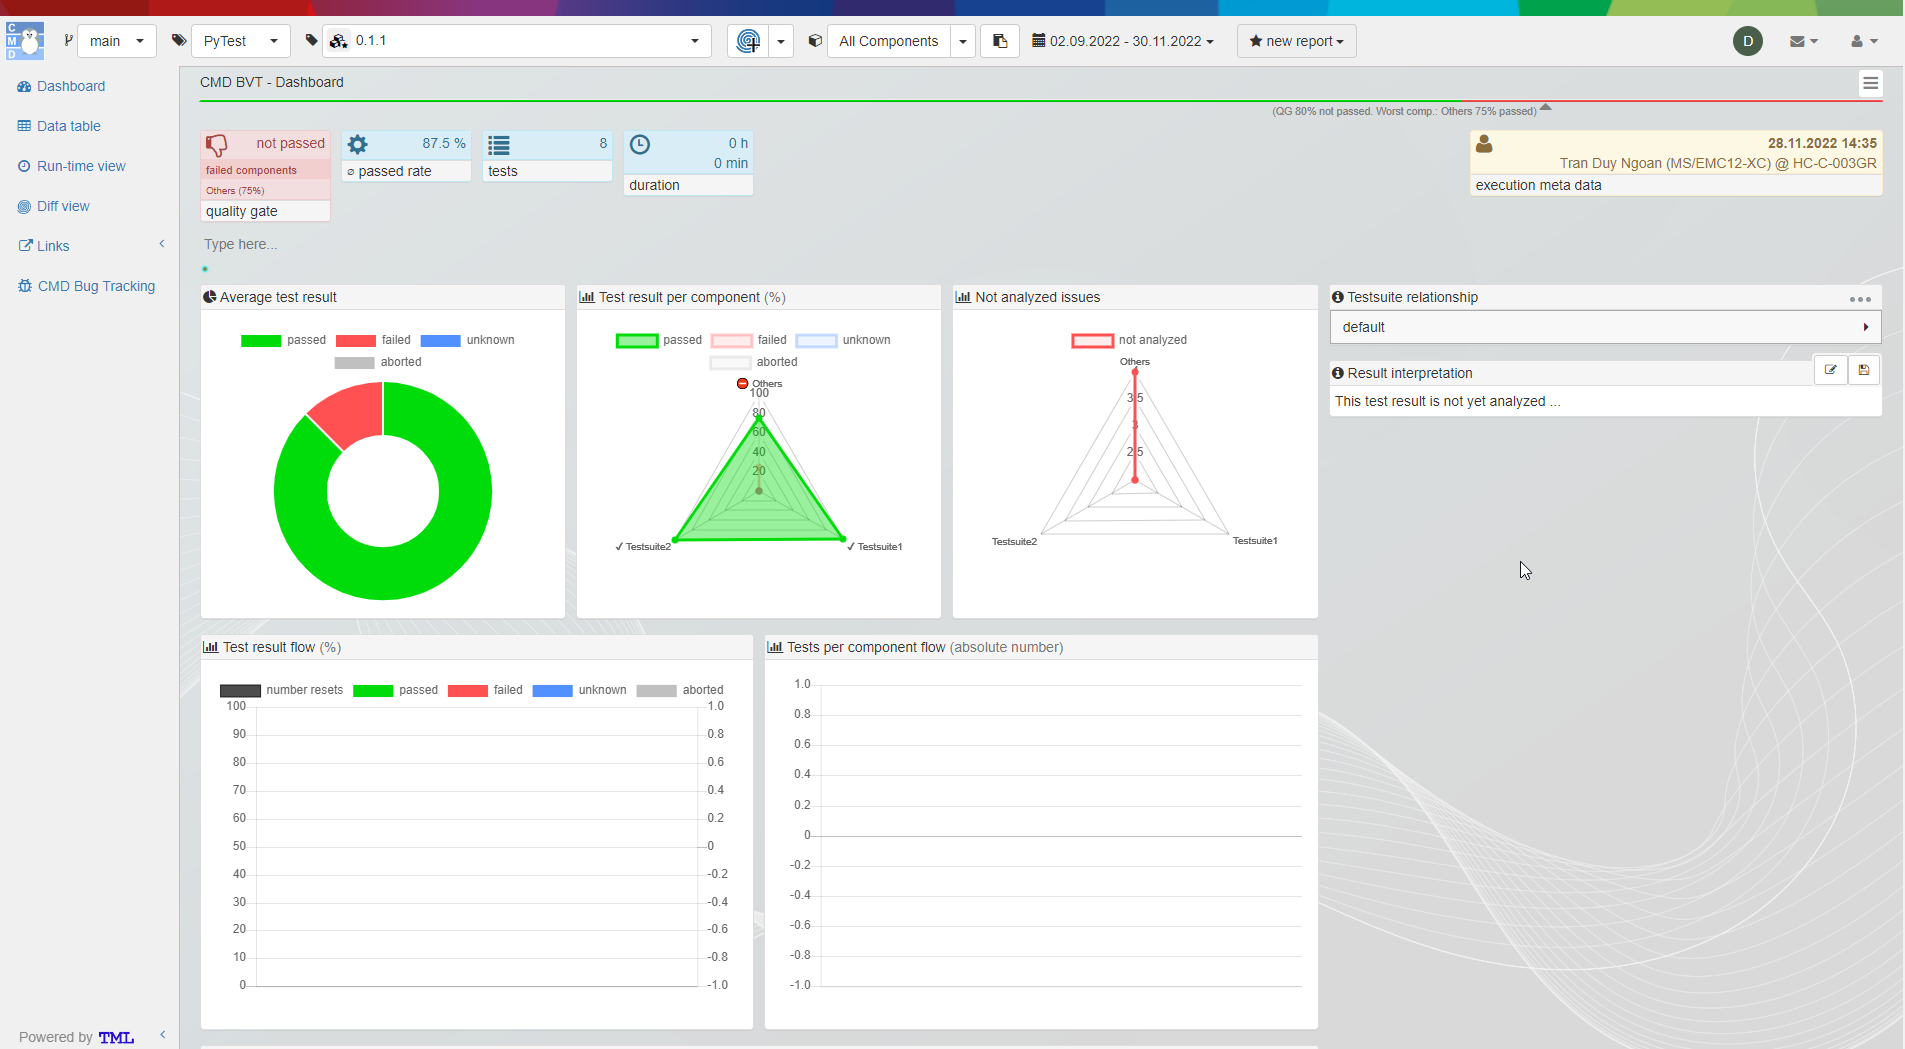
\includegraphics[width=1\linewidth]{./pictures/Dashboard.png}
  \caption{Dashboard view}
\end{figure}

Datatable view:

\begin{figure}[h!]
  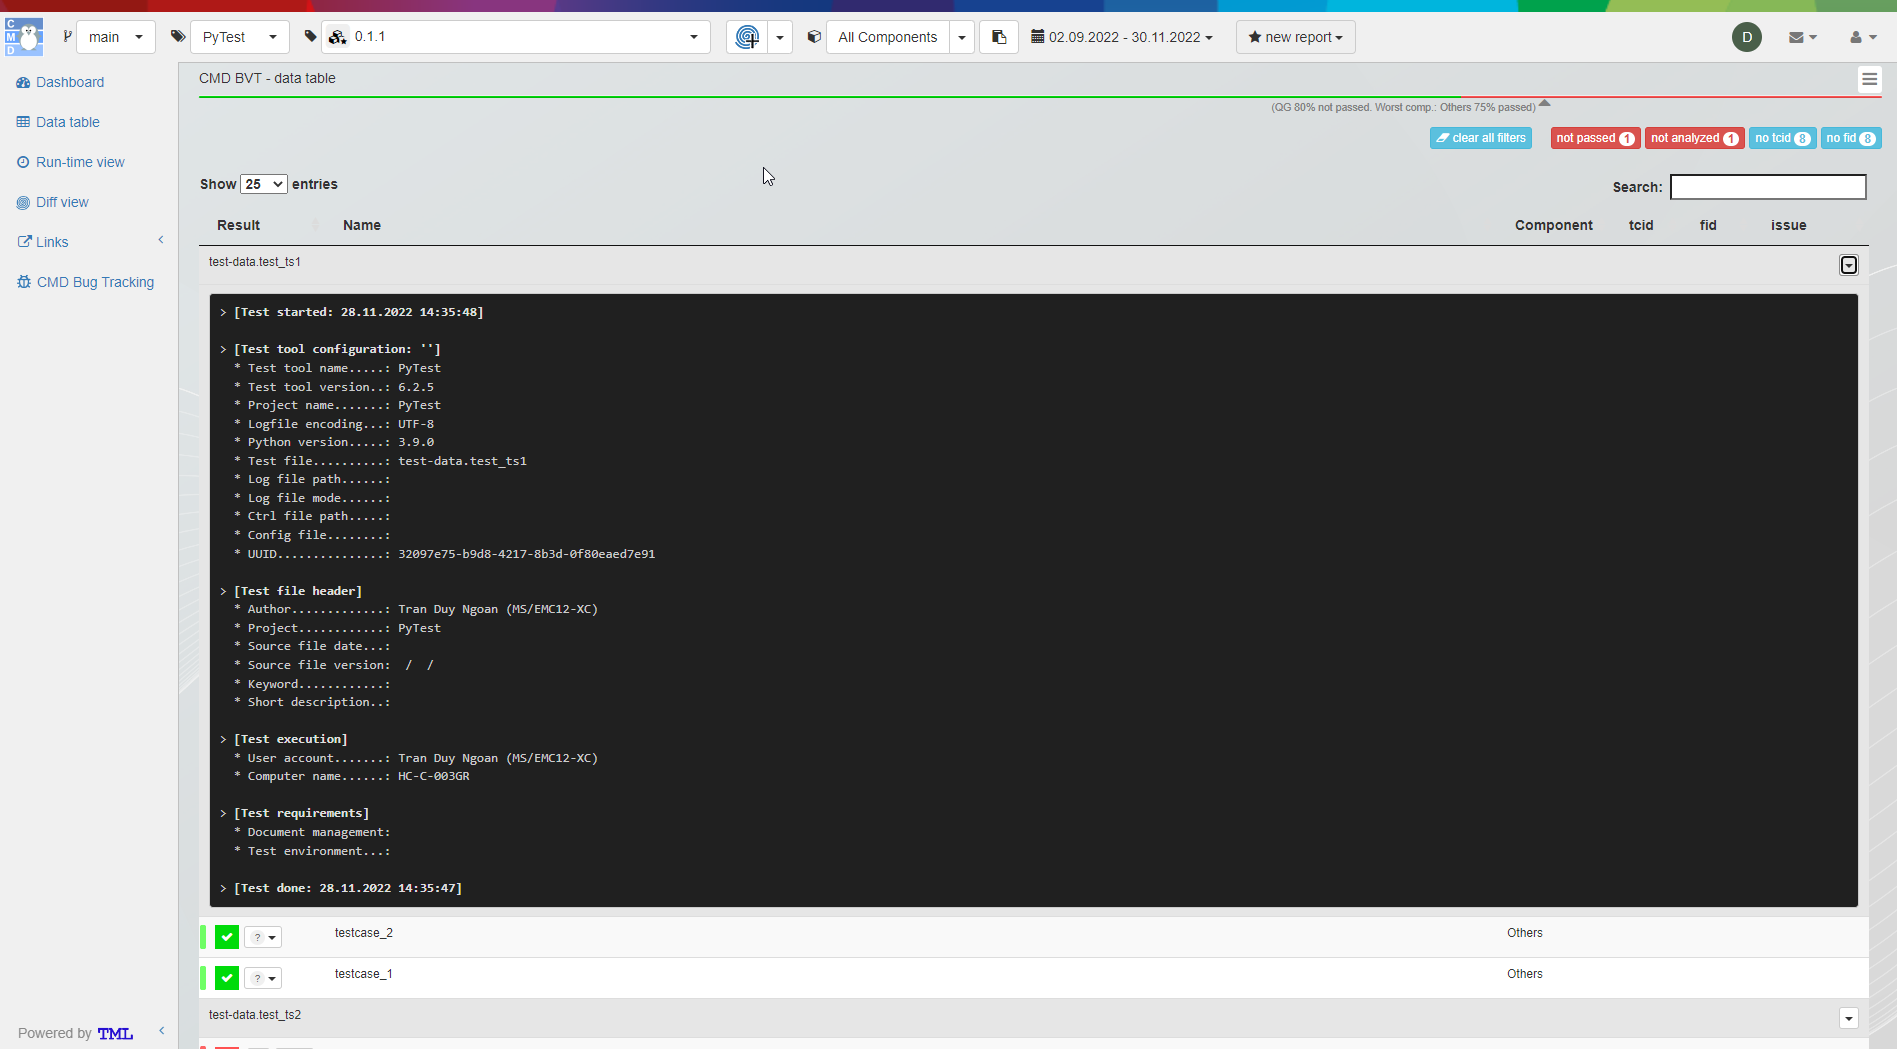
\includegraphics[width=1\linewidth]{./pictures/Datatable.png}
  \caption{Datatable view}
\end{figure}
